% !TEX root = 00_MAIN.tex

\chapter{MTTKRP} \label{sec:mttkrp}

The Matricized Tensor Times Khatri-Rao Product (MTTKRP) operation is a key 
kernel of many tensor decomposition methods.  In CP-ALS, for example,
MTTKRP updates one factor matrix $A$ of a Kruskal tensor using values from
the other factor matrices $B$ and $C$ as follows:
\begin{equation}
\label{eq:mttkrp}
a_{ir} = \sum_{jk \in \X} x_{ijk} b_{jr} c_{kr}, \; i=1,\ldots,I, \; r=1,\ldots,R
\end{equation}

In GCP-SGD, MTTKRP updates factor matrices of a gradient ktensor $\T G$ in a 
similar manner.

\section{Parallel MTTKRP vs. Parallel SpMV} \label{sec:spmv}

The analogy between parallel MTTKRP and parallel sparse matrix-vector
multiplication (SpMV) is strong.   In the SpMV $(\vec a) = X (\vec b)$, 
vector entries of the vector $(\vec a)$ are updated using the values 
of $(\vec b)$:
\begin{equation}
\label{eq:spmv}
a_i = \sum_{j \in \X} x_{ij} b_j.
\end{equation}
 
In parallel SpMV, input vector entries $b_j$ must be communicated to processors 
having nonzeros in column $j$ of the matrix; 
this communication is called an ``expand''
communication.  
The received values are multiplied by the processor's $x_{ij}$.
The resulting products are then summed across matrix rows.
All processors with nonzeros in row $i$ must accumulate their partial
sums into output vector entry $a_i$; this communication operation is 
called a ``fold'' communication.  These expand and fold operations are 
illustrated in Figure~\ref{fig:spmv}.

\begin{figure}[ht]
   \centering
   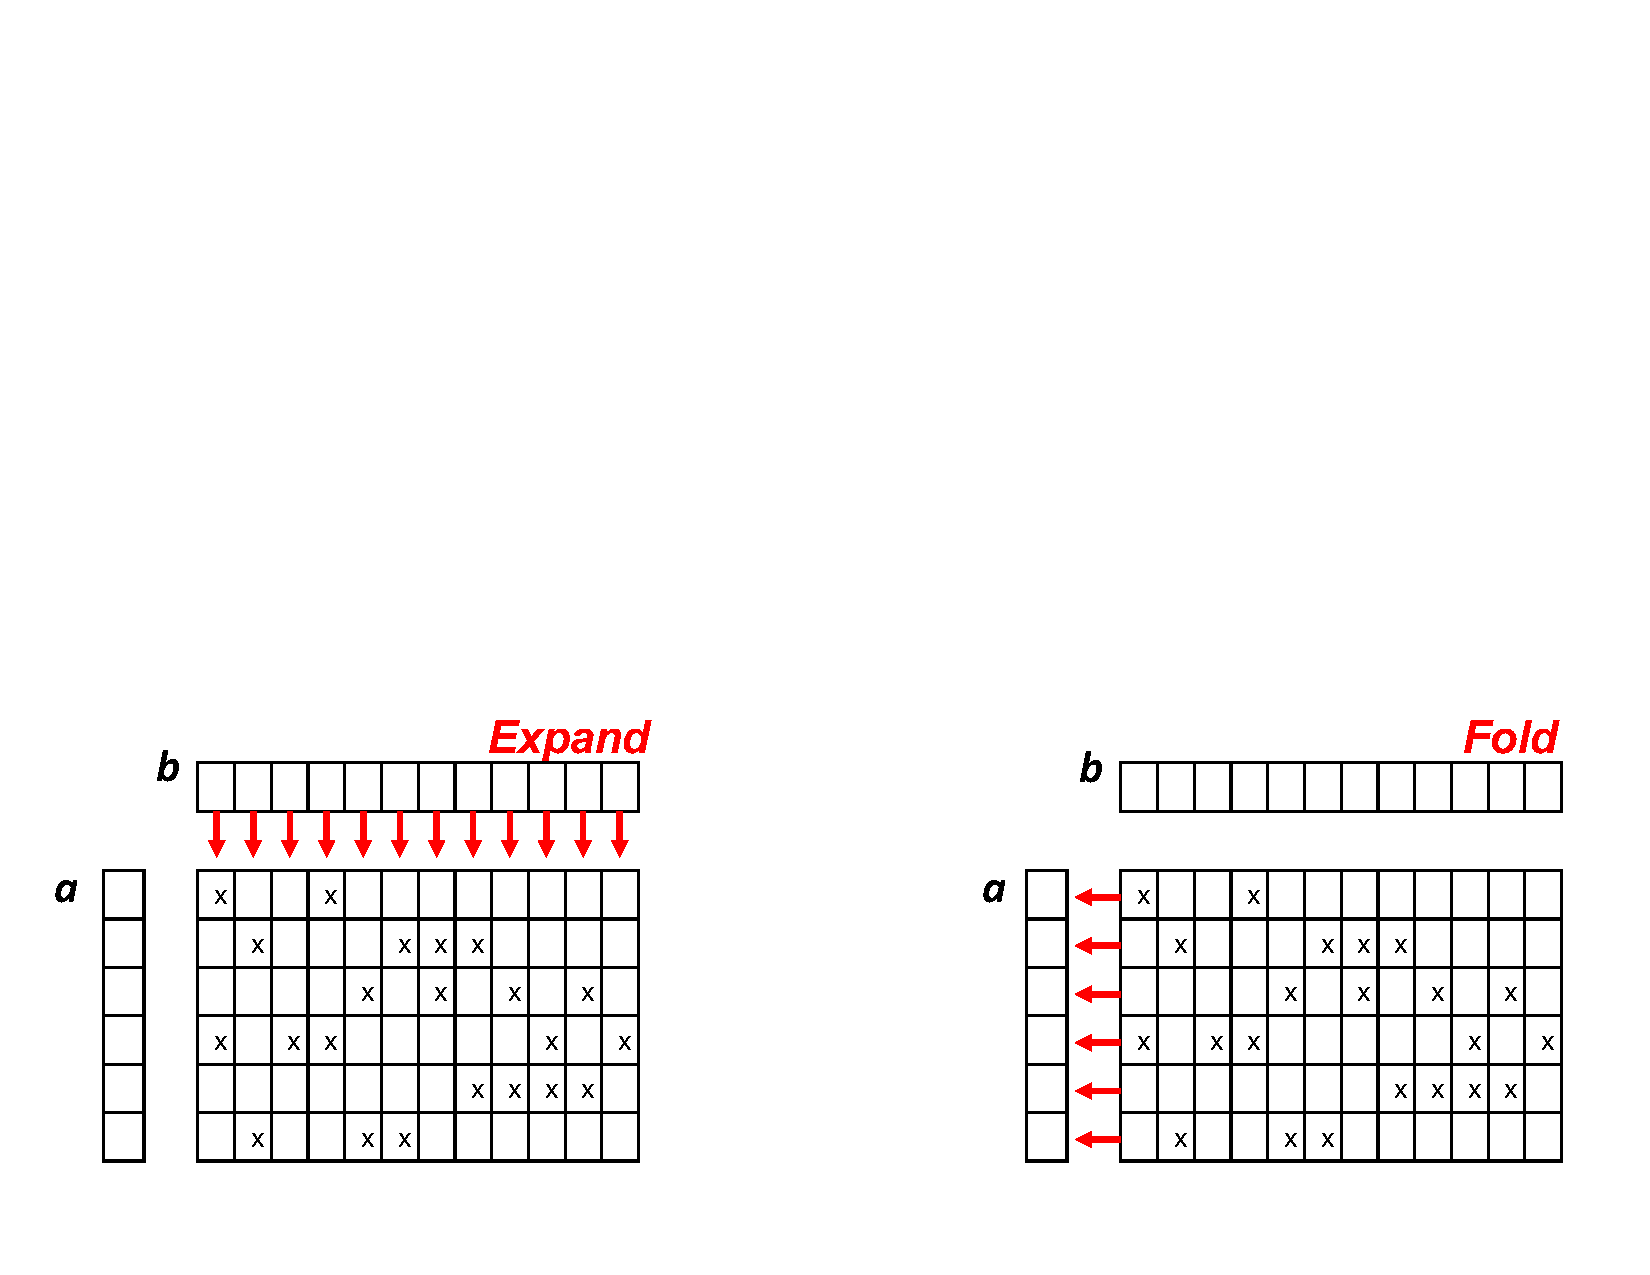
\includegraphics[keepaspectratio=true, width=6.5in]{figs/spmv}
   \caption[The expand and fold communication involved in SpMV]{The expand and fold communication involved in SpMV.  In the expand communication, the input vector entries $b_j$ are communicated to processors with nonzeros in column $j$.
Local products $x_{ij} b_j$ are computed. Then the fold communication 
accumulates partial sums across processors sharing matrix rows $i$ into output
vector entry $a_i$.}
   \label{fig:spmv}
\end{figure}

Parallel MTTKRP requires the same expand and fold communications, as 
illustrated in Figure~\ref{fig:mttkrp}.  In the expand communication,
entries from
factor matrices $B$ and $C$ are communicated to processors with 
corresponding tensor entries.  
Partial sums are then computed within the processor.  
The fold operation then communicates and accumulates
the partial sums into the result factor matrix $A$.

\begin{figure}[ht]
   \centering
   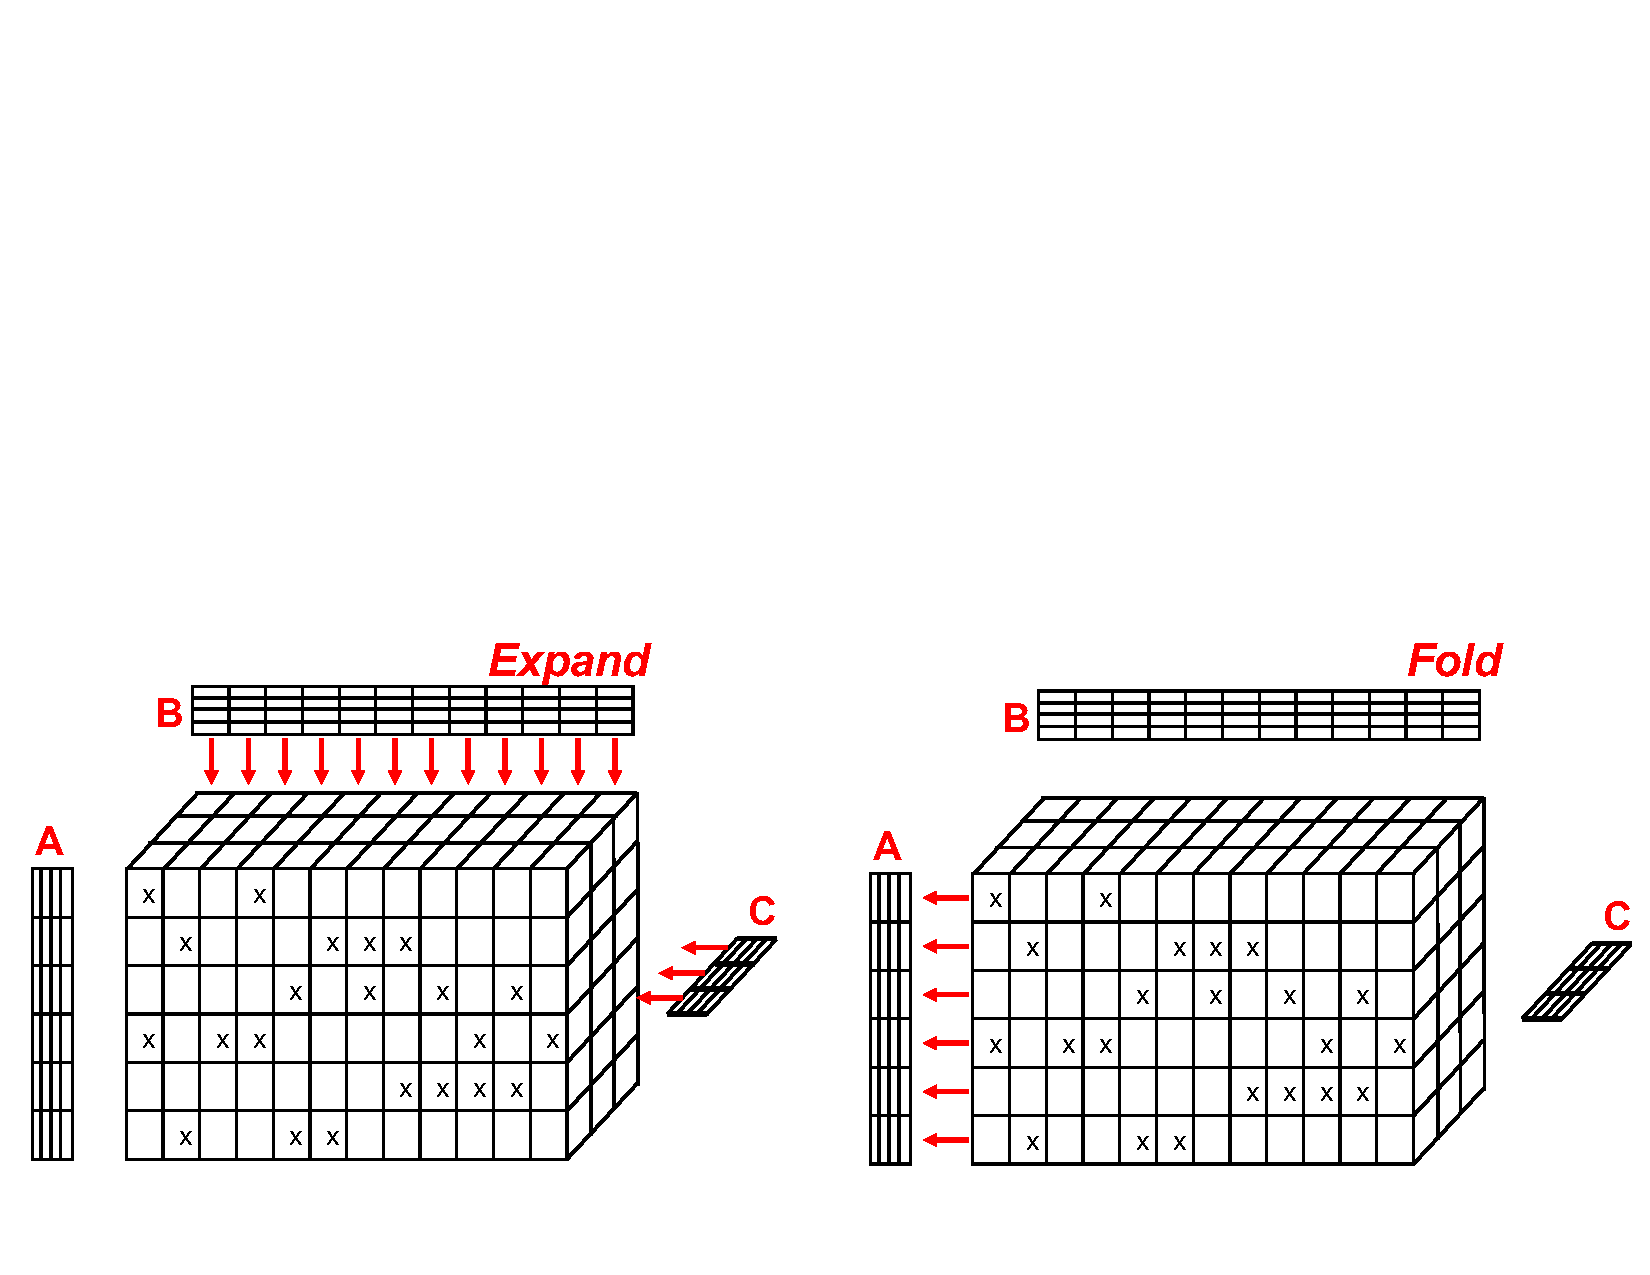
\includegraphics[keepaspectratio=true, width=6.5in]{figs/mttkrp}
   \caption[The expand and fold communication involved in MTTKRP]{The expand and fold communication involved in MTTKRP.  In the expand communication, the entries input factor matrices $B$ and $C$ are communicated to processors with corresponding entries in the tensor $\X$.
Local products $x_{ijk} b_{jr} c_{kr}$ are computed. 
Then the fold communication 
accumulates partial sums across processors into output
factor matrix $A$.}
   \label{fig:mttkrp}
\end{figure}


\section{Implementation}

The MTTKRP implementation in GentenMPI works much like the implementation 
of SpMV in Tpetra.  Here, we'll assume factor matrix $A$ will receive the 
result of the MTTKRP computed from three-way tensor $\X$ and 
factor matrices $B$ and $C$; this scenario is relevant to CP-ALS 
(Chapter~\ref{sec:cpals}).

\begin{enumerate}
\item MTTKRP requires a {\tt distSystem} object $D$ constructed from the tensor
$\X$ and a Kruskal tensor with the factor matrices $A$, $B$, and $C$.  
During construction of the $D$, its internal factor matrices $\hat A$, 
$\hat B$, and $\hat C$ are updated 
via communication using the {\tt Import} objects in each mode.
This update constitutes the ``expand'' communication, and brings to each 
processor the factor matrix entries in each mode corresponding to the 
indices of the processor's $x_{ijk}$ entries.

\item \label{mttkrp:local} Local products are computed within each processor.  The processor loops
over its owned tensor entries $x_{ijk}$ and multiplies them by the associated
entries $\hat b_{jr}$ and $\hat c_{kr}$, accumulating the results in 
$\hat a_{ir}$.  This operation is a triply nested loop, first over the 
$N_p$ tensor entries on a processor, 
then over tensor modes, and then over the rank $R$.

\item \label{mttkrp:fold} After completion of the local computation, $D$'s {\tt Import} object 
associated with $A$ communicates values from $\hat A$ 
back to $A$, with contributions from multiple 
processors summed into $A$.  This operation is the ``fold'' communication.

\item \label{mttkrp:lastupdate} Once $A$ is updated by all processors, 
the accrued values of $A$ can be communicated back to $\hat A$ to keep the 
internal factor matrices up-to-date with actual factor matrix values.
\end{enumerate}

For GCP-SGD (Chapter~\ref{sec:gcp}), 
the result of the MTTKRP with $B$ and $C$ is not stored in 
$A$, but rather, is stored in an additional factor matrix $G$.  In this case,
additional storage $\hat G$ is used to receive the result of the MTTKRP in
step~\ref{mttkrp:local}, and $\hat G$ is communicated to $G$ in 
step~\ref{mttkrp:fold}.  Step~\ref{mttkrp:lastupdate} is not needed since
neither $\hat A$ nor $A$ is changed in the MTTKRP.

\section{Column-major vs Row-major}

The default layout of data in Tpetra's {\tt MultiVector} class
is column-major ({\tt Kokkos::LayoutLeft}); that is, for an $I \times R$ factor 
matrix, the first vector of length $I$ is stored, followed by the second
vector of length $I$, and so on.  This layout is convenient for some linear
solvers that need to access a single vector or a subset of vectors of a 
given multivector.
However, in MTTKRP, all $R$ factor matrix
entries for a given index $i$ are accessed together in step~\ref{mttkrp:local} 
above.  The default layout causes strided memory acceses that can lead to 
poor cache performance.

A better layout for MTTKRP is row-major ({\tt Kokkos::LayoutRight}), in
which all $R$ entries for a given index $i$ are stored contiguously in 
memory.  Thus, GentenMPI uses a modified Tpetra {\tt MultiVector} that 
uses row-major storage; these modifications were trivial and did not interfere
with Tpetra's communication of multivector data values.

Figure~\ref{fig:layouts} shows the difference in performance using 
column-major vs row-major layouts.  This example was run on one processor
of Sandia's SkyBridge cluster with 2.6GHz Intel Sandy Bridge processors.
It uses the \emph{delicious-4d} tensor from the FROSTT~\cite{FROSTT} tensor collection,
a $532,924 \times 17,262,471 \times 2,480,308 \times 1443$ tensor with 140 million
nonzeros.  With rank $R=8$, the difference in MTTKRP time between column-
and row-major layouts is visible; column-major layout requires 1.7 times more
execution time per MTTKRP.  With larger values of
$R$, the difference becomes even more significant, with column-major layout
taking 3.4 times longer than row-major layout for $R=32$.


\begin{figure}[ht]
   \centering
   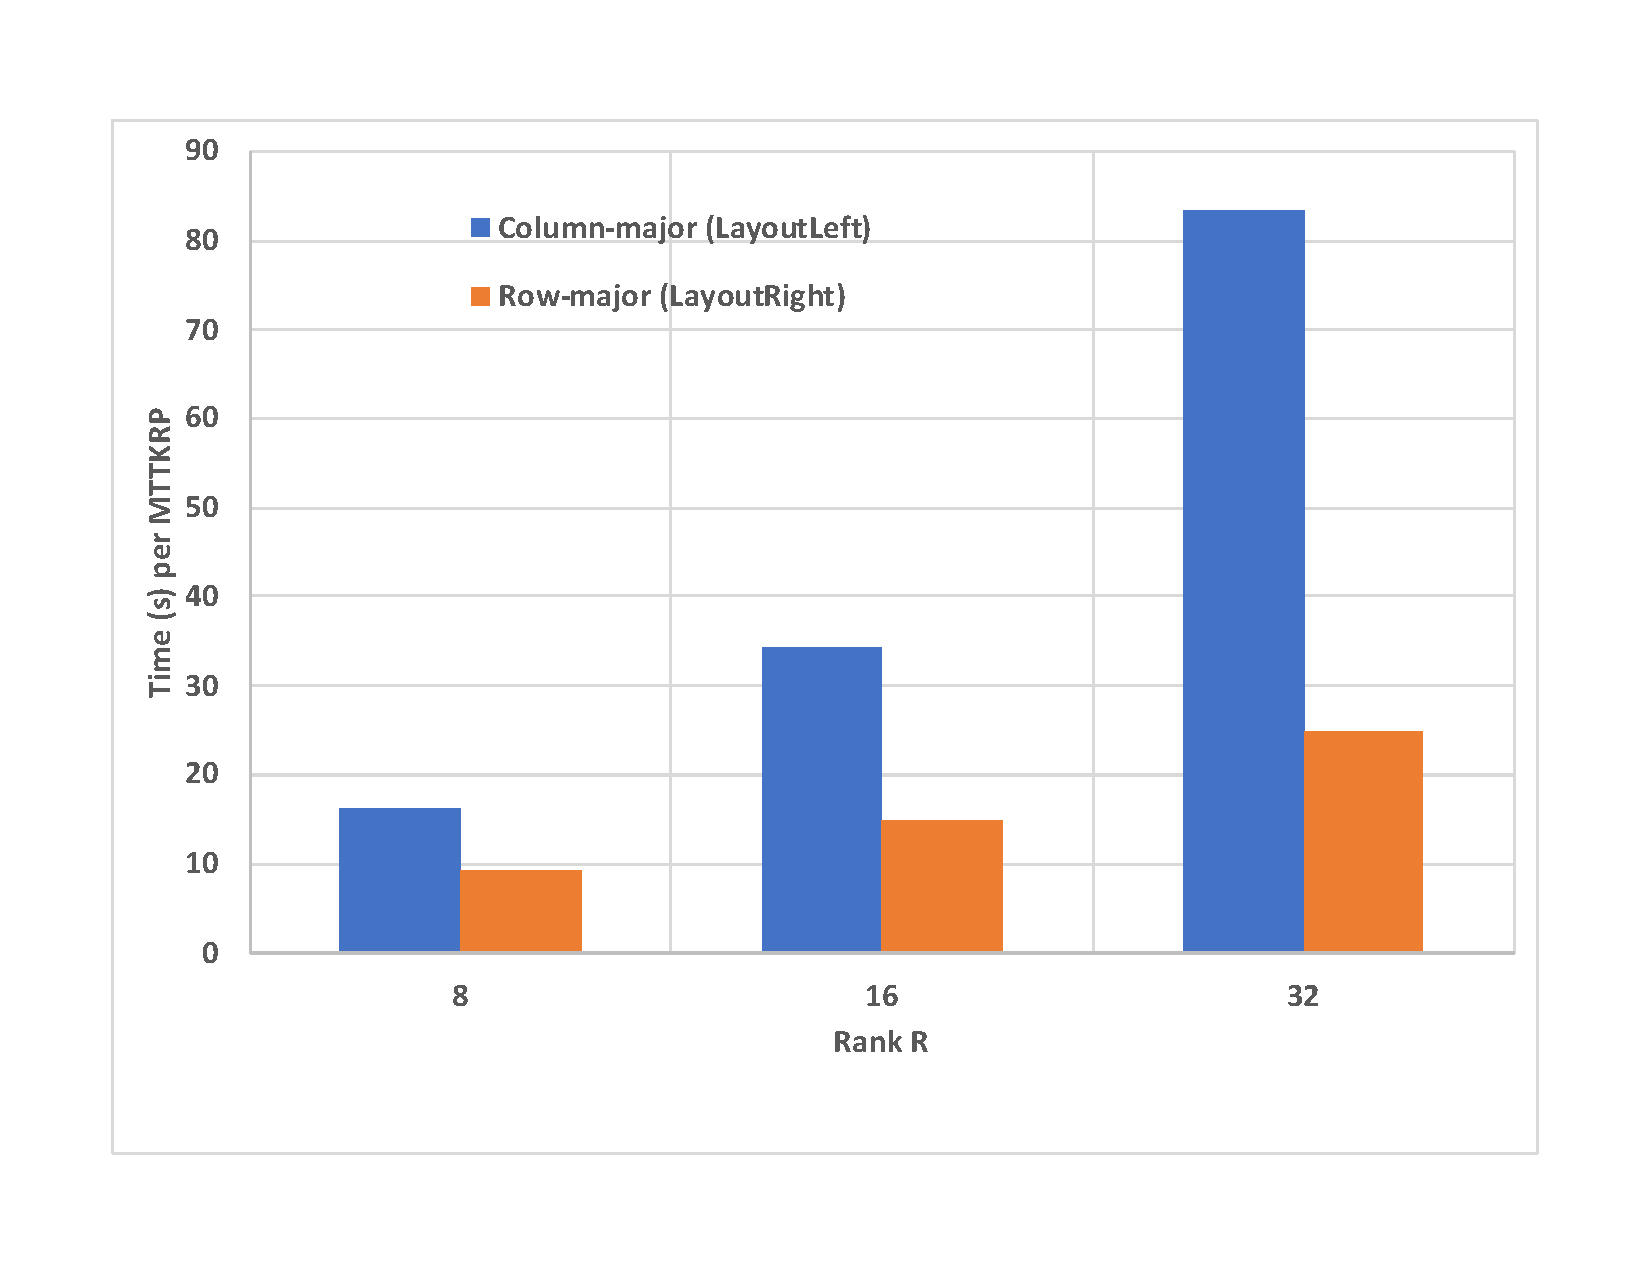
\includegraphics[keepaspectratio=true, width=4.5in]{figs/layouts}
   \caption[MTTKRP times using column- and row-major layout of factor matrices]{MTTKRP times using column-major (LayoutLeft) and row-major
(LayoutRight) layout of the factor matrices. (\emph{delicious-4d}
tensor, rank $R=8,16,32$)}
   \label{fig:layouts}
\end{figure}

For all experiments in the remainder of this report, GentenMPI uses
row-major (\texttt{Kokkos::LayoutRight}) layout for all factor matrices.
